 
%
\documentclass[aspectratio=169]{beamer}
%\documentclass[aspectratio=1610]{beamer}
%\documentclass[aspectratio=149]{beamer}
%\documentclass[aspectratio=54]{beamer}
%\documentclass[aspectratio=43]{beamer}
%\documentclass[aspectratio=32]{beamer} 


\usepackage[utf8]{inputenc}                                      
\usepackage[T1]{fontenc}  
\usepackage[polish]{babel} 

\usepackage{graphicx}
\usepackage{epstopdf}

\ifxetex  % XeLaTeX
   \usepackage{fontspec}
   \defaultfontfeatures{Mapping=tex--text}   % to support TeX conventions like dashes etc
   \usepackage{xltxtra} % extra customisation for XeLaTeX
%   \setsansfont{Linux Biolinum O}
%   \setmainfont[Ligatures={Common,TeX}, Numbers={OldStyle}]{Linux Libertine O}
%      \setsansfont{Barlow Semi Condensed}
%      \setmainfont{PT Serif}
%   \setsansfont{Ubuntu}
%   \setmonofont{Ubuntu Mono}

\else  % LaTeX
   \usepackage[T1]{fontenc}
   \usepackage[utf8]{inputenc}
%   \usepackage[osf,tt=false]{libertine}
\fi


\uselanguage{polish}
\languagepath{polish}
\deftranslation[to=polish]{Definition}{Definicja}
\deftranslation[to=polish]{Example}{Przykład}

\usetheme[sectionpage=progressbar,subsectionpage=progressbar,block=fill,background=light]{metropolis}





\usepackage{indentfirst}
%\usepackage{graphicx} 
%\usepackage{hyperref}
%\usepackage{booktabs}
%\usepackage{tikz}
%\usetikzlibrary{arrows}
%\usepackage{pgfplots}
%\usepackage{subfigure}
%\usepackage{color}
%\usepackage{listings}
%\usepackage{filecontents}
%\usepackage{fontawesome5}
%\usepackage{amssymb}



%\usepackage[backend=bibtex,style=alphabetic]{biblatex}
%plain --> \usepackage[style=numeric]{biblatex}
%abbrv --> \usepackage[style=numeric,firstinits=true]{biblatex}
%unsrt --> \usepackage[style=numeric,sorting=none]{biblatex}
%alpha --> \usepackage[style=alphabetic]{biblatex}

%\newrobustcmd*
\newcommand%
{\footfullcitenomark}{%
  \AtNextCite{%
    \let\thefootnote\relax
    \let\mkbibfootnote\mkbibfootnotetext}%
  \footfullcite}
\newcommand{\stopka}[1]{\footfullcitenomark{#1}}  



\newcommand{\hcancel}[1]{%
   \tikz[baseline=(tocancel.base)]{
      \node[inner sep=0pt,outer sep=0pt] (tocancel) {#1};
      \draw[red, thick] (tocancel.south west) -- (tocancel.north east);
   }%
}%


%%%%%%%%%%%%%%%%%%%%%%%%%%%%

 

%\setbeamertemplate{footline}
%    {\begin{beamercolorbox}[sep=1ex]{author in head/foot}
%      \rlap{\textit{\insertshorttitle}}\hfill\insertauthor\hfill\llap{\insertframenumber}%
%      \end{beamercolorbox}%
%}

 
\newcommand{\HUGE}{\fontsize{35}{30}\selectfont}
%\newcommand{\veryHuge}{\fontsize{65}{55}\selectfont}
\newcommand{\veryHuge}{\fontsize{45}{40}\selectfont}

\usepackage{color}
\definecolor{cornflowerblue}{cmyk}{0.65, 0.13, 0   , 0   }

\newcommand*{\myfont}{\fontfamily{LinuxLibertineT-OsF}\selectfont}

\newcommand{\cytowanie}[1]{%
   \raisebox{-0.2cm}{\myfont\color{blue}\veryHuge «}\myfont\Large #1\raisebox{-0.2cm}{\myfont\color{blue}\veryHuge »}
} 



\title[Klasyfikacja mocap z LSTM]{Automatyczna klasyfikacja danych motion capture przy użyciu sieci LSTM}
\subtitle{Prezentacja projektu}
\author{Tymoteusz Mucha, Jakub Szafarczyk, Konrad Wnuk}
\institute[PolSl]{
\includegraphics[scale=0.25]{graf/politechnika_sl_logo_poziom_pl}}


%\date{23 marca 2021}
%\logo{
\includegraphics[scale=0.2]{graf/politechnika_sl_logo_pion_pl.eps}}

\frenchspacing

\begin{document}
\maketitle

%%%%%%%%%%%%%%%%%%%%%%%%%%%%%%%%%%%%%%%%%%%%%%%%%%%%%%%%%%%%%%%%%%%%%%%%
\begin{frame}[fragile]{Czym jest motion capture}
	\begin{itemize}
		\item Rejestracja ruchu w przestrzeni 3D.
		\item Wynik: sekwencja pozycji markerów lub stawów w czasie.
		\item Każda klatka -- ,,szkielet'' opisany wektorem współrzędnych.
		\item Technologie: optyczne (Vicon), IMU, mechaniczne, magnetyczne.
		\item Zastosowania: animacja, biomechanika, sport, rehabilitacja.
	\end{itemize}
	
\end{frame}
	
\begin{frame}[fragile]{Sekwencja klatek chodu}
	\centering
	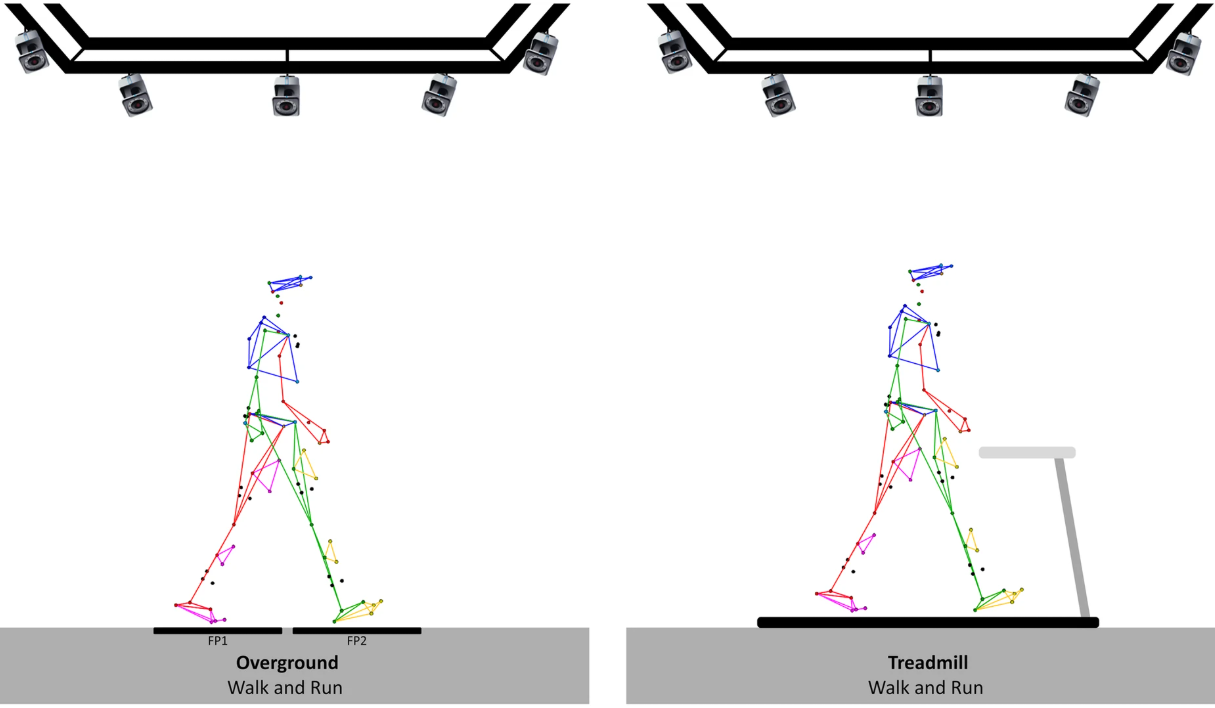
\includegraphics[height=0.85\textheight, width=\textwidth, keepaspectratio]{graf/walk_sequence.png}
\end{frame}


%%%%%%%%%%%%%%%%%%%%%%%%%%%%%%%%%%%%%%%%%%%%%%%%%%%%%%%%%%%%%%%%%%%%%%%%
\begin{frame}[fragile]{Sieć LSTM -- opis sieci}
	\begin{itemize}
		\item LSTM = Long Short-Term Memory, wariant rekurencyjnej sieci neuronowej.
		\item Zaprojektowana do uczenia się zależności w sekwencjach.
		\item Rozwiązuje problem zanikającego gradientu klasycznych RNN.
		\item Trzy bramki sterują przepływem informacji w komórce:
		\begin{itemize}
			\item \textbf{forget} -- co wyrzucić z pamięci,
			\item \textbf{input} -- co dopisać,
			\item \textbf{output} -- co wypuścić dalej.
		\end{itemize}
	\end{itemize}
	
	\begin{block}{Dlaczego LSTM dla mocap}
		ruch to sekwencja czasowa -- LSTM modeluje relacje między klatkami
	\end{block}
\end{frame}


%%%%%%%%%%%%%%%%%%%%%%%%%%%%%%%%%%%%%%%%%%%%%%%%%%%%%%%%%%%%%%%%%%%%%%%%
\begin{frame}[fragile]{Architektura sieci}
	\begin{itemize}
		\item \textbf{Stacked LSTM} -- trzy warstwy:
		\begin{itemize}
			\item LSTM (15 neuronów, \texttt{return\_sequences=True}),
			\item LSTM (15 neuronów) -- pogłębienie modelu,
			\item Dense + softmax -- klasyfikator wyjściowy.
		\end{itemize}
		\item Funkcja straty: MSE.
		\item Optymalizator: Adam (lr = 0{,}001).
		\item Wejście: tensor \texttt{(sample\_size, n\_features)}.
		\item Wyjście: rozkład prawdopodobieństwa nad klasami (one-hot).
	\end{itemize}
\end{frame}

\begin{frame}[fragile]{Schemat warstw sieci LSTM}
	% >>> OBRAZEK: schemat warstw sieci (z keras.utils.plot_model) <<<
	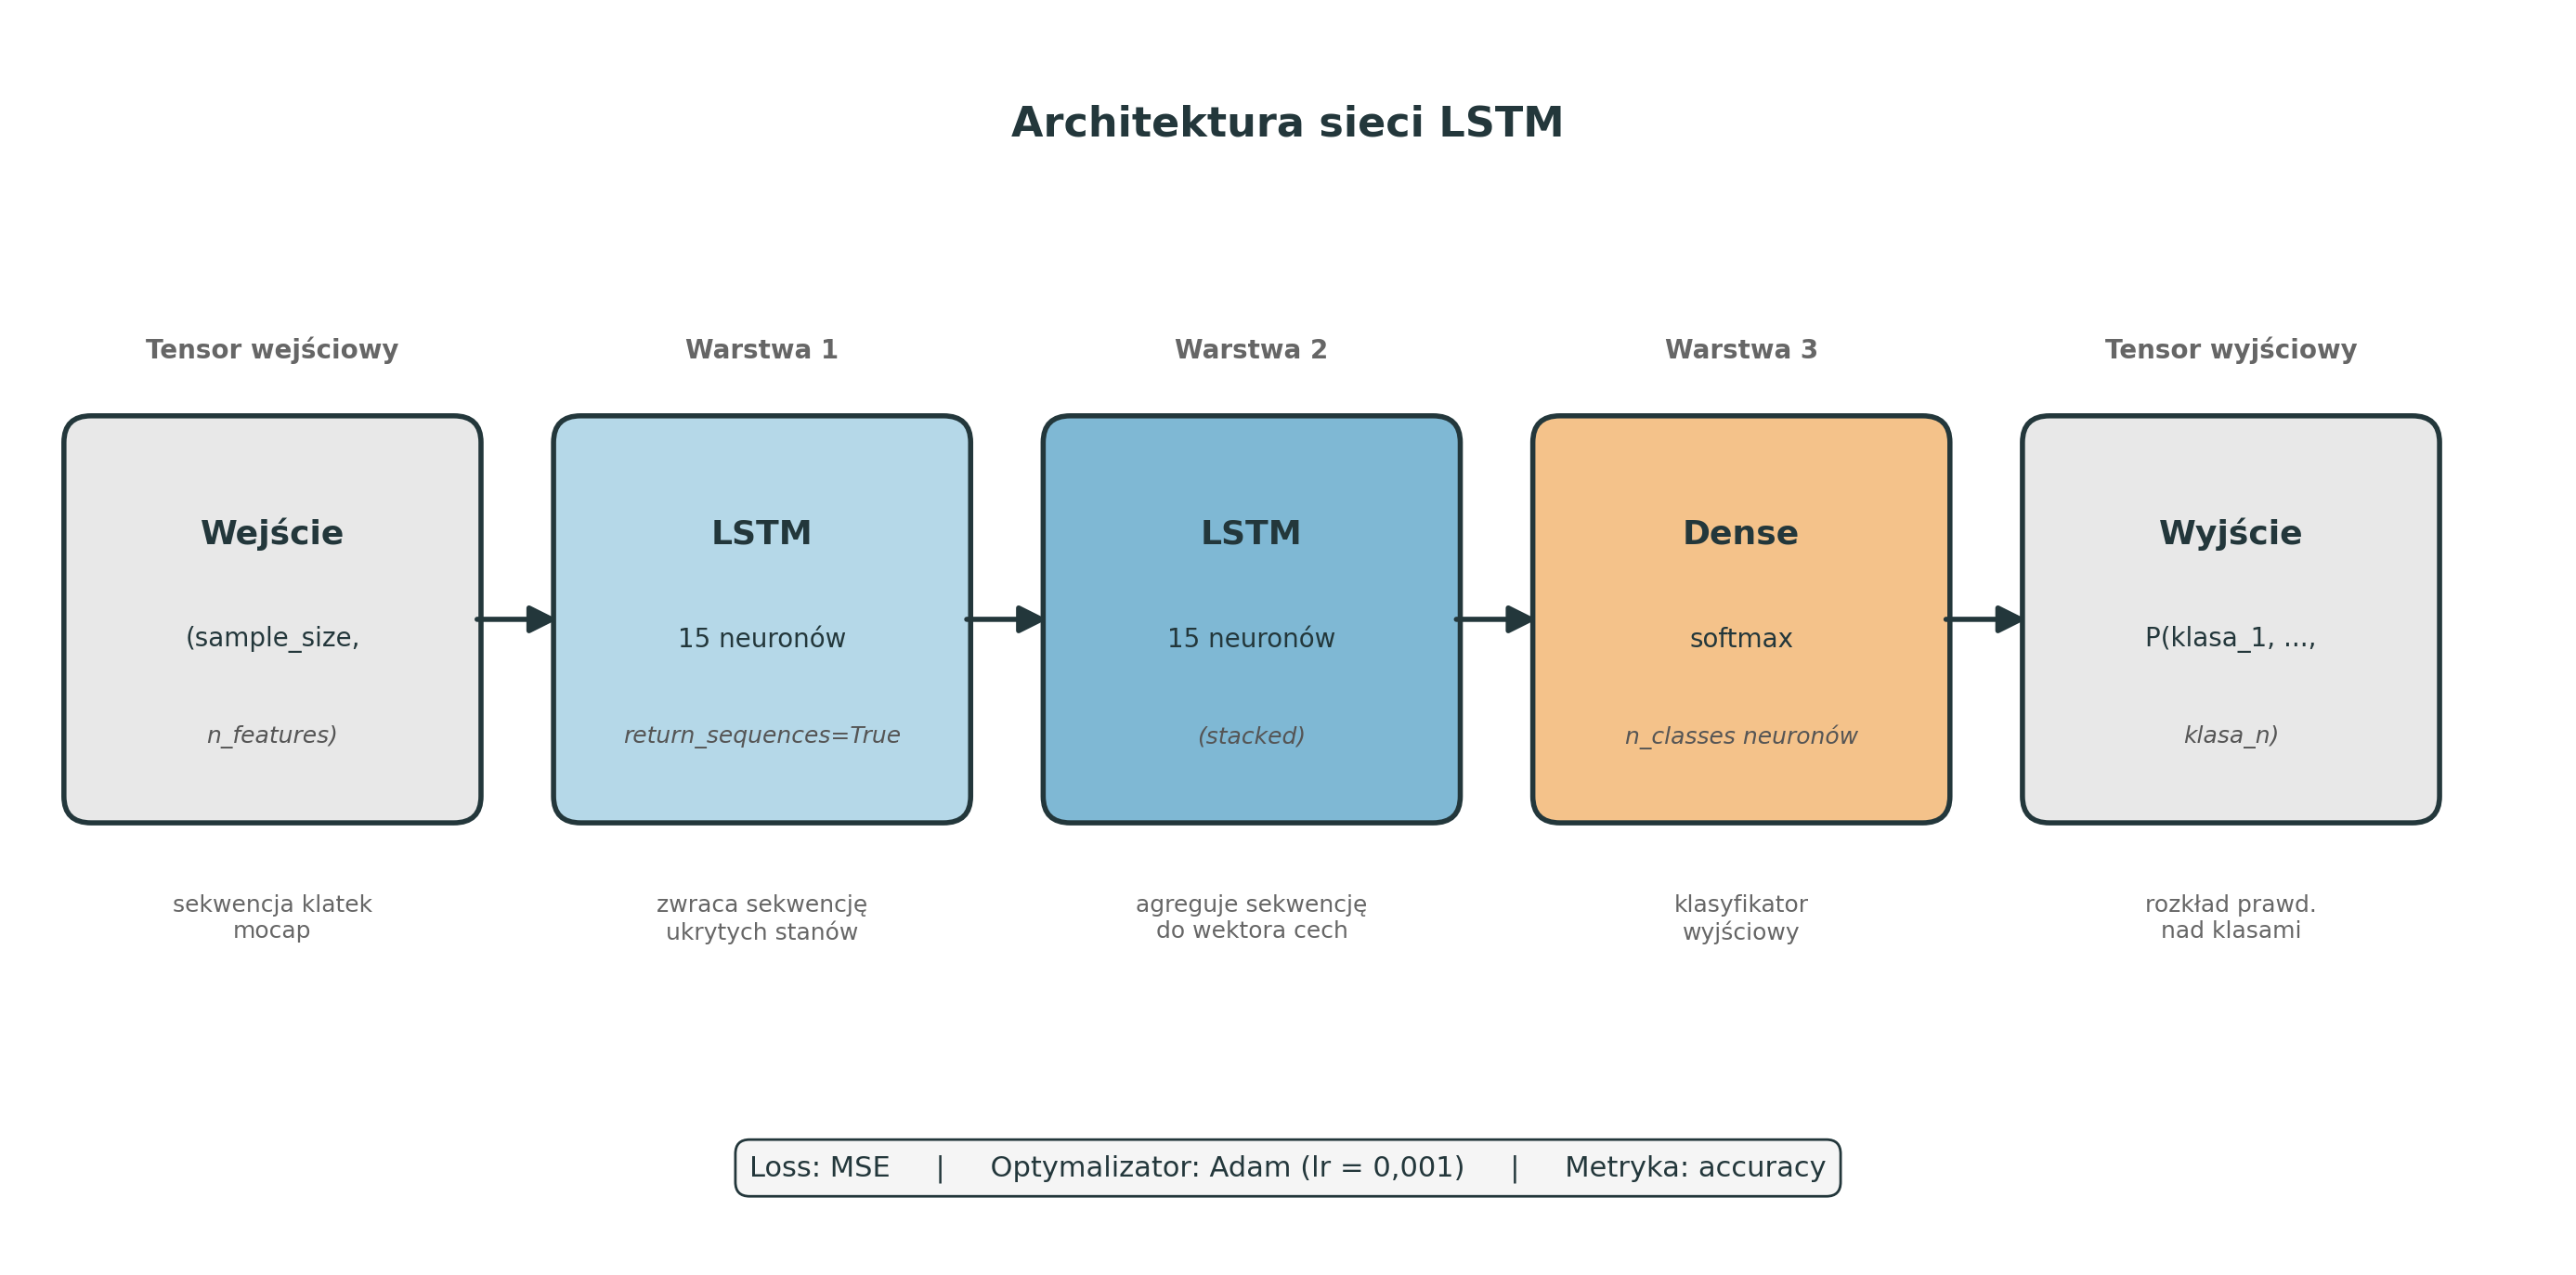
\includegraphics[height=0.85\textheight, width=\textwidth, keepaspectratio]{graf/network.png}
\end{frame}


%%%%%%%%%%%%%%%%%%%%%%%%%%%%%%%%%%%%%%%%%%%%%%%%%%%%%%%%%%%%%%%%%%%%%%%%
\begin{frame}[fragile]{Parametry i warianty modelu}
	\begin{itemize}
		\item \textbf{Rozmiar okna} (\texttt{sample\_size}): 1, 5, 10, 15, 20 klatek.
		\item \textbf{Liczba klas (ontologia)}: 2 (chód/bieg) -- multi-label.
		\item \textbf{Głębokość sieci}: liczba warstw LSTM.
		\item \textbf{Liczba neuronów}: 15, 32, 64, 128.
		\item \textbf{Funkcja straty}: MSE vs categorical crossentropy.
		\item \textbf{Agregacja}: moda predykcji okien w pliku.
	\end{itemize}
	
	\vspace{1em}
	\begin{block}{Wniosek z literatury (da Silva et al., 2019)}
		dla 9 klas accuracy $\sim$50\,\%, dla 4 dobrze zróżnicowanych klas $>$95\,\%
	\end{block}
\end{frame}


%%%%%%%%%%%%%%%%%%%%%%%%%%%%%%%%%%%%%%%%%%%%%%%%%%%%%%%%%%%%%%%%%%%%%%%%
\begin{frame}[fragile]{Zbiór danych -- źródło}
	\textbf{Riglet et al., 2024 -- Scientific Data (Nature)}\\
	\emph{,,3D motion analysis dataset of healthy young adult volunteers walking and running on overground and treadmill''}
	
	\vspace{0.8em}
	\begin{itemize}
		\item 30 zdrowych ochotników (28 $\pm$ 6 lat).
		\item 63 markery refleksyjne (Conventional Gait Model 2.5).
		\item System Vicon, 18 kamer, 100 Hz.
		\item Dwie sesje na uczestnika (odstęp 7 dni).
		\item Chód: 3 prędkości; bieg: 2 prędkości.
		\item Środowiska: \emph{overground} i bieżnia.
	\end{itemize}
\end{frame}

\begin{frame}[fragile]{Zbiór danych -- rozmieszczenie markerów}
	\centering
	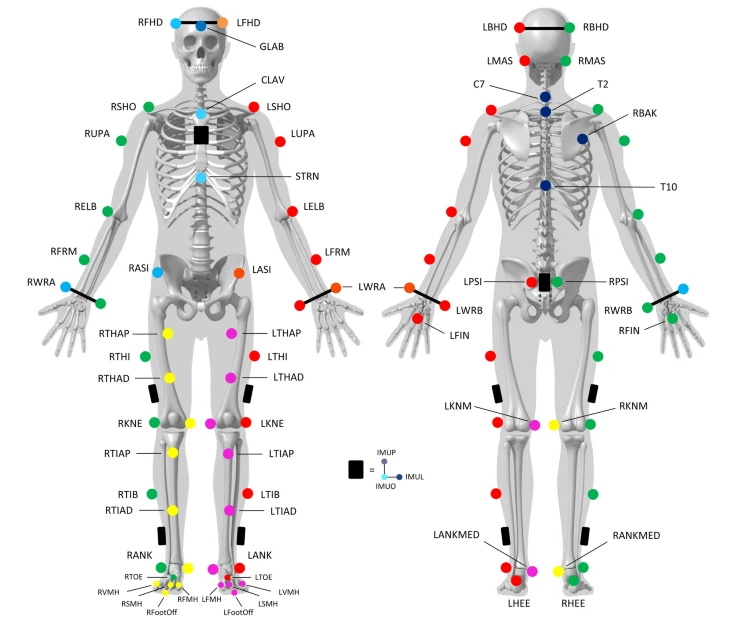
\includegraphics[height=0.85\textheight, keepaspectratio]{graf/cgm_markers.png}
\end{frame}


%%%%%%%%%%%%%%%%%%%%%%%%%%%%%%%%%%%%%%%%%%%%%%%%%%%%%%%%%%%%%%%%%%%%%%%%
\begin{frame}[fragile]{Zbiór danych -- skala i format}
	\begin{itemize}
		\item Liczba zarejestrowanych cykli ruchu:
		\begin{itemize}
			\item chód \emph{overground}: 4\,840
			\item chód na bieżni: 18\,159
			\item bieg \emph{overground}: 2\,931
			\item bieg na bieżni: 18\,945
		\end{itemize}
		\item Format \textbf{C3D} -- standard biomechaniki (binarny).
		\item Format \textbf{CSV} -- tekstowy, czytelny w pandas/Excel.
		\item Wersje: \emph{raw} oraz \emph{post-processed}.
		\item Struktura: \texttt{ID/Sesja/Próba/Prędkość/Dane/Plik}.
	\end{itemize}
	
	\vspace{0.5em}
	\begin{block}{Skala}
		ponad 44\,000 cykli ruchu = duży zbiór treningowy dla LSTM
	\end{block}
\end{frame}


%%%%%%%%%%%%%%%%%%%%%%%%%%%%%%%%%%%%%%%%%%%%%%%%%%%%%%%%%%%%%%%%%%%%%%%%
\begin{frame}[fragile]{Wykorzystanie danych w projekcie}
	\begin{itemize}
		\item Klasyfikacja rodzaju chodu.
		\item Klasyfikacja płci.
		\item Klasyfikacja identyfikacji uczestnika.
	\end{itemize}
	
	\vspace{0.5em}
	\textbf{Wejście do sieci:}
	\begin{itemize}
		\item wektor współrzędnych XYZ wybranych markerów,
		\item normalizacja: centrowanie wokół miednicy,
		\item podział na okna o długości \texttt{sample\_size}.
	\end{itemize}
\end{frame}


%%%%%%%%%%%%%%%%%%%%%%%%%%%%%%%%%%%%%%%%%%%%%%%%%%%%%%%%%%%%%%%%%%%%%%%%
\begin{frame}[fragile]{Narzędzia i biblioteki}
	\begin{itemize}
		\item \textbf{Środowisko:} Python 3, Jupyter Notebook
		\item \textbf{Sieć neuronowa:} TensorFlow + Keras
		\item \textbf{Dane mocap:} ezc3d / BTK (pliki C3D)
		\item \textbf{Przetwarzanie:} NumPy, pandas
		\item \textbf{Ewaluacja:} scikit-learn (metryki, podział zbioru)
		\item \textbf{Wizualizacja:} matplotlib, seaborn, Mokka
	\end{itemize}
	
	\vspace{0.8em}
	% >>> Logos technologii (analogicznie jak w szablonie e-skoroszyt) <<<
	% Aby je dodać: wrzucić pliki PNG do graf/ i odkomentować poniższe linie.
	 
\includegraphics[height=1.5cm]{graf/Python.png}\hspace{0.6cm}
	 
\includegraphics[height=1.5cm]{graf/Tensorflow.png}\hspace{0.6cm}
	 
\includegraphics[height=1.5cm]{graf/Keras.png}\hspace{0.6cm}
	 
\includegraphics[height=1.5cm]{graf/Numpy.png}\hspace{0.6cm}
	 
\includegraphics[height=1.5cm]{graf/Pandas.png}\hspace{0.6cm}
	 
\includegraphics[height=1.5cm]{graf/Scikit_learn.png}
\end{frame}


%%%%%%%%%%%%%%%%%%%%%%%%%%%%%%%%%%%%%%%%%%%%%%%%%%%%%%%%%%%%%%%%%%%%%%%%
\begin{frame}[fragile]{Plan eksperymentów}
	\begin{itemize}
		\item Wczytanie danych C3D/CSV.
		\item Normalizacja i podział na okna czasowe.
		\item Podział train/val/test na poziomie uczestnika.
		\item Trening sieci LSTM dla różnych konfiguracji.
		\item Ewaluacja: accuracy, precision, recall, F1, macierz pomyłek.
		\item Porównanie wariantów hiperparametrów.
	\end{itemize}
	
	\vspace{1em}
	\begin{block}{Oczekiwane wyniki}
		rodzaj chodu $>$95\,\%, płci 80--90\,\%, identyfikacja uczestnika 70--85\,\%
	\end{block}
\end{frame}

%%%%%%%%%%%%%%%%%%%%%%%%%%%%%%%%%%%%%%%%%%%%%%%%%%%%%%%%%%%%%%%%%%%%%%%%
\begin{frame}[fragile]{Literatura i~źródła}
	\textbf{Artykuł referencyjny:}
	\begin{itemize}
		\item da Silva, R., Ondřej, J., Smolic, A.\\
		\emph{Using LSTM for Automatic Classification of Human Motion Capture Data}.\\
		VISIGRAPP 2019, s.~236--243.\\
		DOI: \texttt{10.5220/0007349902360243}
	\end{itemize}
	
	\vspace{0.8em}
	\textbf{Zbiór danych:}
	\begin{itemize}
		\item Riglet, L. i~in.\\
		\emph{3D motion analysis dataset of healthy young adult volunteers walking and running on overground and treadmill}.\\
		Scientific Data 11, 556 (2024).\\
		\url{https://www.nature.com/articles/s41597-024-03420-y}
	\end{itemize}
\end{frame}

%\begin{frame}{\LaTeX\ifxetex, \XeLaTeX\fi}
%
%Szablon można skompilować zarówno \LaTeX em, jak i Xe\LaTeX em. Będą użyte inne rodziny fontów. 
%
%Xe\LaTeX\ \ifxetex(\XeLaTeX) \fi używa fontu Fira, \LaTeX\ używa domyślnego fontu.
%
%\ifxetex
%\XeLaTeX\ ŵʂþıɛʁɑ ƒɒɲŧɣ ưɳɨƙơɖɔʍɜ, ʥɪęʞï ʈɘɱʊ
%ɰɵʐna ƥìʃɐɕ ʬ ʌįɞɬʉ ʝęʑỷķæçɧ. 
%
%źdźbło żółć fuŝĥoraĵo æbletræ ¡¿piña?! smršť ſoß 
%ťęľěģŕåþħ
%şœșŋøŵý 
%äße 
%γλῶττα Ἀτρεΐδης· ὃ γὰρ ἦλθε θοὰς
%љубав међа 
%ѕвезда їжак
%à ă ä á â ǎ ą å ā ã ạ ȧ æ
%ì ĩ ī ĭ í į ı i ị ï ǐ î ɨ ỉ
%ò ö õ ō ó ő ø ŏ ǒ ô ǫ 
%è é ê ě è é ê ë ē ĕ ė ę ě ȅ ȩ ȇ ḕ ḕ ḗ ḗ ḙ ḛ ḝ ẹ ẻ ẽ ề ế ể ễ ề ế ể ễ
%ǥ ƀ ħ ŧ đ ð p þ b 
%\fi 
%\end{frame}
%
%\subsection{Podsekcja 1}
%
%\begin{frame}{Tytuł}
%\begin{itemize}
%\item raz
%\item dwa
%\item trzy \alert{alert}
%\end{itemize}
%\end{frame}
%
%\subsection{Podsekcja 2}
%
%
%
%\begin{frame}{Wzory}
%\begin{align*}
%A = \int_{-\infty}^{0} \exp \left( - \frac{(x-m)^2}{2\sigma^2}\right) dx
%\end{align*}
%\end{frame}
%
%\begin{frame}{Grafiki}
%\begin{center}
%
\includegraphics[width=\textwidth]{./graf/politechnika_sl_logo_poziom_pl.eps}
%\end{center}
%\end{frame}
%
%\section{Bloki}
%
%\begin{frame}{Bloki}
%\begin{definition}[Koercja]
%Spiralna dyslokacja efemerydy Kuppelweisera
%\end{definition}
%
%\begin{exampleblock}{Przykład}
%Przykładowo, gdy $x < \pi$, wtedy $\sum_{i=1}^{n} \frac{1}{i}$.
%\end{exampleblock}
%
%\begin{block}{Tytuł bloku}
%Zawartość bloku …
%\end{block}
%
%\begin{alertblock}{Uwaga!}
%Memento mori!
%\end{alertblock}
%
%\end{frame}
%
%\begin{frame}[standout]
%slajd negatywowy
%\end{frame}
%
\maketitle
%
%\appendix 
%
%\begin{frame}{Dodatek}
%\begin{enumerate}
%\item Slajdy w dodatku nie są wliczane do liczby stron prezentacji. 
%\item Nie mają numerów stron.
%\item Nie wpływają na pasek postępu slajdów.
%\end{enumerate}
%\end{frame}

\end{document}

